% Use only LaTeX2e, calling the article.cls class and 12-point type.

\documentclass[12pt]{article}

% Users of the {thebibliography} environment or BibTeX should use the
% scicite.sty package, downloadable from *Science* at
% http://www.sciencemag.org/authors/preparing-manuscripts-using-latex
% This package should properly format in-text
% reference calls and reference-list numbers.

\usepackage{scicite}

\usepackage{times}
\usepackage{amsmath, amssymb}

% The preamble here sets up a lot of new/revised commands and
% environments.  It's annoying, but please do *not* try to strip these
% out into a separate .sty file (which could lead to the loss of some
% information when we convert the file to other formats).  Instead, keep
% them in the preamble of your main LaTeX source file.


%%%%%% taken from papaja-created ver
\usepackage{csquotes}
\usepackage{graphicx}
  \usepackage[unicode=true]{hyperref}
\usepackage{threeparttablex}            % Lets threeparttable work with longtable

% The following parameters seem to provide a reasonable page setup.

\topmargin 0.0cm
\oddsidemargin 0.2cm
\textwidth 16cm
\textheight 21cm
\footskip 1.0cm


%The next command sets up an environment for the abstract to your paper.

\newenvironment{sciabstract}{%
\begin{quote} \bf}
{\end{quote}}


%EY: to add S to figure number in supplementary materials
\newcommand{\beginsupplement}{%
        \setcounter{table}{0}
        \renewcommand{\thetable}{S\arabic{table}}%
        \setcounter{figure}{0}
        \renewcommand{\thefigure}{S\arabic{figure}}%
     }

%EY: color for comments
\usepackage[usenames, dvipsnames]{color}

\definecolor{Red}{RGB}{255,0,0}
\definecolor{Green}{RGB}{10,200,100}
\definecolor{Blue}{RGB}{10,100,200}
\definecolor{Orange}{RGB}{255,153,0}

\newcommand{\ejy}[1]{\textcolor{Red}{[ejy: #1]}}
\newcommand{\ndg}[1]{\textcolor{Green}{[ndg: #1]}}
\newcommand{\mht}[1]{\textcolor{Blue}{[mht: #1]}}
\newcommand{\mcf}[1]{\textcolor{Orange}{[mcf: #1]}}

%EY: add packages
 \usepackage{lscape}
 \usepackage{array, booktabs, makecell}
 \usepackage{siunitx, mhchem}


% Include your paper's title here

% \title{Polite speech emerges from competing pressures to be (and look) informative and kind}
\title{Polite speech emerges from competing social goals}
% speakers' competing social goals?

% Place the author information here.  Please hand-code the contact
% information and notecalls; do *not* use \footnote commands.  Let the
% author contact information appear immediately below the author names
% as shown.  We would also prefer that you don't change the type-size
% settings shown here.

\author
%{Erica J. Yoon,$^{1\ast}$ Michael Henry Tessler,$^{1\ast}$ Noah D. Goodman,$^{1}$ Michael C. Frank$^{1}$\\
%\\
%\normalsize{$^{1}$Department of Psychology, Stanford University}\\
%\\
%\normalsize{$^\ast$These authors contributed equally to this work.}
%
%}
{Erica J. Yoon,$^{1\ast\dagger}$ Michael Henry Tessler,$^{1\ast}$ Noah D. Goodman,$^{1}$ Michael C. Frank$^{1}$\\
\\
\normalsize{$^{1}$Department of Psychology, Stanford University,}\\
\normalsize{450 Serra Mall, Stanford, CA 94305.}
\\
\normalsize{$^\ast$These authors contributed equally to this work.}
\\
\normalsize{$^\dagger$To whom correspondence should be addressed; E-mail: ejyoon@stanford.edu.}
}

% Include the date command, but leave its argument blank.

\date{}

%%%%%%%%%%%%%%%%% END OF PREAMBLE %%%%%%%%%%%%%%%%
\begin{document}

% Double-space the manuscript.

\baselineskip24pt

% Make the title.

\maketitle

% Place your abstract within the special {sciabstract} environment.

\begin{sciabstract}
Language is a remarkably efficient tool for information transfer. Yet to be polite, speakers often behave in ways that are at odds with this goal, making statements that are imprecise or even outright false. Why? We show that polite speech emerges from competing goals: to be informative, to be kind, and to \emph{appear} to be both of these. We formalize this tradeoff using a probabilistic model of speakers' utterance choice, which predicts human judgments with high accuracy. This utility-theoretic approach to speech acts takes a step towards explaining the richness and subtlety of social language.
\end{sciabstract}

% In setting up this template for *Science* papers, we've used both
% the \section* command and the \paragraph* command for topical
% divisions.  Which you use will of course depend on the type of paper
% you're writing.  Review Articles tend to have displayed headings, for
% which \section* is more appropriate; Research Articles, when they have
% formal topical divisions at all, tend to signal them with bold text
% that runs into the paragraph, for which \paragraph* is the right
% choice.  Either way, use the asterisk (*) modifier, as shown, to
% suppress numbering.

%%%%%%%%%%%%%%%%%%
%%%%% Introduction %%%%%%%
%%%%%%%%%%%%%%%%%%

We don't always say what we're thinking. \enquote{Close the
window!} could be sufficient, but instead we add \enquote{can you please\ldots{}?}
or \enquote{would you mind\ldots{}?}
Rather than tell an
uncomfortable truth, we lie (\enquote{Your dress looks great!}) and
prevaricate (\enquote{Your poem was so appropriate to the occasion}).
Such utterances are puzzling for standard views of language use, which
see communication as the transfer of information from a sender to a
receiver \cite{buhler1934, shannon1948, jakobson1960, frank2012}. On these views, transfer ought to be efficient and
accurate: The speaker should choose a succinct utterance  to convey
what the speaker knows \cite{grice1975, searle1975},
and the information transferred should be accurate and truthful
to the extent of the speaker's knowledge. Polite speech --
like the examples above -- violates these basic expectations: It is inefficient,
underinformative, and sometimes outright false. Why are we
polite?

Theories of politeness explain deviations from optimal information
transfer by assuming that speakers take into account informational \emph{and} social concerns.
These concerns have been described as polite maxims \cite{leech1983} or social norms \cite{ide1989},
but the most influential account relies on the notion of \emph{face} \cite{brown1987, goffman1967}.
Under the face-based framework for polite language, interactants seek to be liked,
approved, and related to (\emph{positive face}) as well as to maintain
their freedom to act (\emph{negative face}).
Though intuitively appealing, the theory does not describe when face should be prioritized over other concerns (e.g., information transfer) nor when face-saving should yield indirect (e.g., \enquote{Your cake could use a bit of salt}) vs. false (\enquote{It's tasty}) statements.
Further, a mutually-understood notion of face introduces additional complexity: Speakers sometimes may not want to preserve the listener's face genuinely but only to be \emph{seen} as doing so, hence appearing to be socially apt and saving their own face, which may lead to a different decision from that based on genuine desires to be kind or informative.
What is needed is a precise theory of these goals and how they trade off.

%The theory, however, does not articulate how these communicative goals should trade off with
%one another.
%For example, it is unclear when the desire to save face
%will motivate statements that are outright false (\enquote{Your cake is
%delicious!}) versus indirect (\enquote{It could use a bit of salt}), and
%when face-saving should be prioritized over other concerns (e.g.,
%helpful information transfer).
%Both inefficient indirect speech and untruthful lies in communication
%are then the result of speakers' strategic choices relative to possible
%face threats.
%The face-based framework for polite language use provides an intuitive
%and appealing explanation of many types of polite speech, but it


%%%%%%%%%%%%%%%%%%
%%%%%% Model %%%%%%%
%%%%%%%%%%%%%%%%%%

To address this challenge, we develop a utility-theoretic model, quantifying tradeoffs between the different communicative goals. In our model, speakers attempt to maximize a set of competing
utilities: an informational utility, derived via effective
information transmission; a social utility, derived by being kind (giving the listener utility); and a self-presentational utility, derived
by being perceived as valuing information transfer or kindness.
Speakers then choose utterances on the basis of their
expected utility.

Utilities are weighed within a Rational Speech Act (RSA) model that
takes a probabilistic approach to pragmatic reasoning in language \cite{frank2012, goodman2016}. Speakers are modeled as agents
who choose utterances by reasoning about their effects on a listener
relative to their cost, while listeners are modeled as inferring
interpretations by reasoning about speakers and their goals.  RSA models have been used to understand a wide variety of complex
linguistic behaviors \cite{lassiter2017adjectival, kao2014, kao2015}, and are part of a broader class of models instantiating the idea that human social cognition can be approximated via reasoning about others as rational agents who act to maximize their subjective utility \cite{baker2009action,jara2016naive, liu2017ten}.

\begin{figure}
\centering
  \makebox[\textwidth]{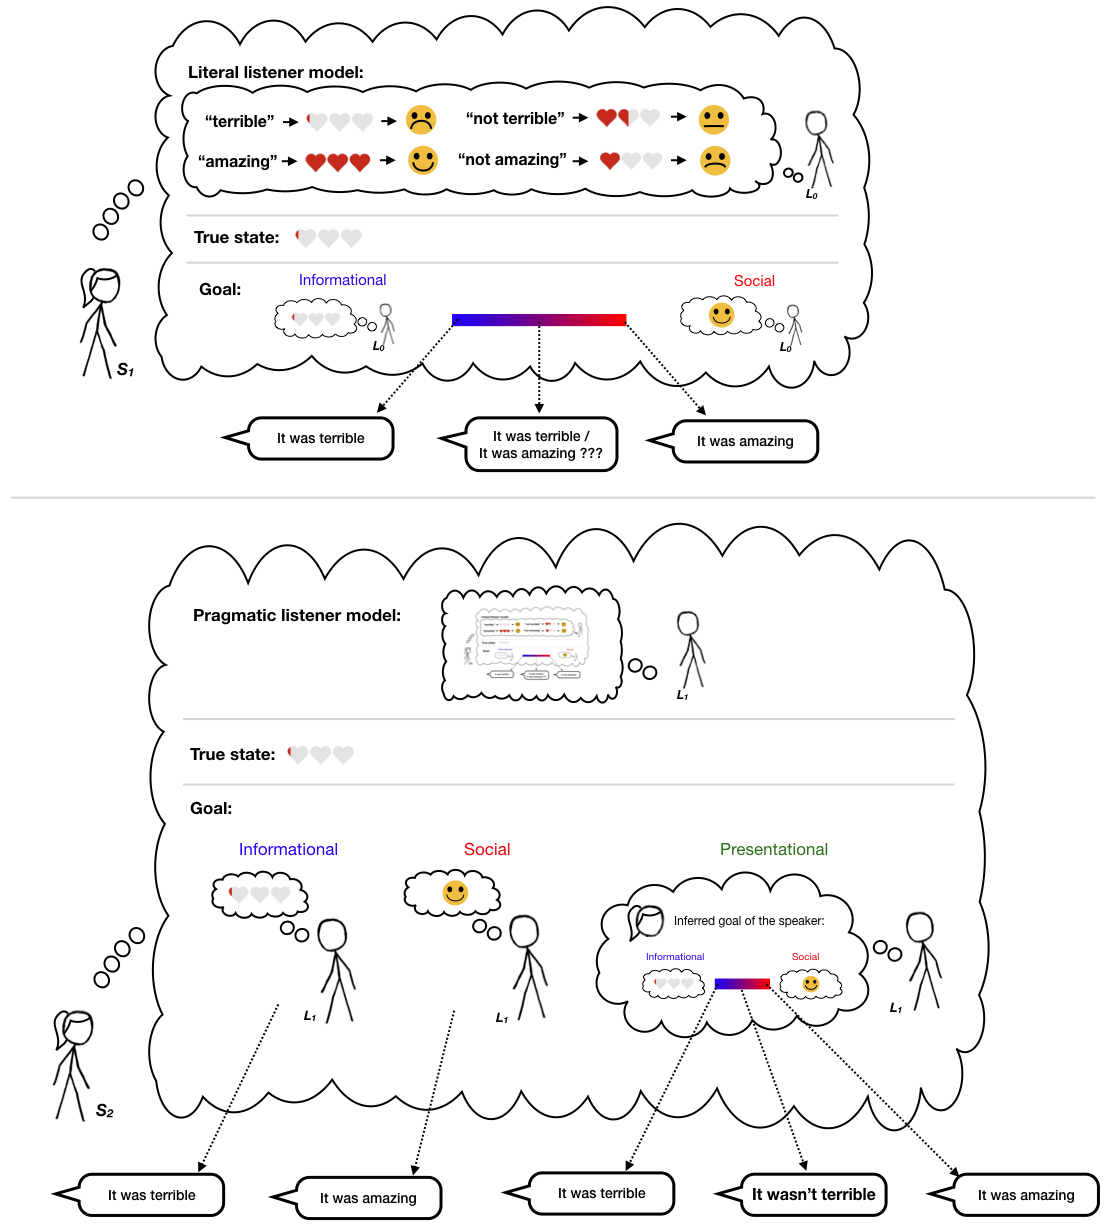
\includegraphics[width=0.8\textwidth]{fig/model}}
\caption{\label{fig:model}Diagram of the model: The pragmatic speaker observes the true state and determines her goal between three utilities (informational, social, and presentational), and produces an utterance.
}
\end{figure}

RSA models are defined recursively such that speakers reason about
listeners, and vice versa. By convention, we index this recursion such that a pragmatic listener \(L_1\) reasons about the intended meaning
and goals a speaker \(S_1\) would have had in order to produce a particular
utterance.
\(S_1\) produces utterances by reasoning about a \enquote{literal listener} \(L_0\), modeled as attending only to the literal meanings of words
(rather than their pragmatic implications), hence grounding the
recursion.
Our current target is a model of a polite speaker
\(S_2\), who reasons about what utterance to say to \(L_1\) by
considering the set of utilities described above (Figure
\ref{fig:model}).

We evaluate our model on its ability to predict human utterance choices in situations where polite language use is expected. Imagine Bob recites a poem he wrote and asks Ann for her opinion.
Ann (\(S_2\)) produces an utterance \(w\) based on the true state of the world \(s\) (the rating Bob's recital deserved) and a set of goal weights
\(\hat{\phi}\), that determine how Ann prioritizes each goal.
Ann's production decision is softmax, which interpolates between
maximizing and probability matching (via parameter \(\lambda_{S_2}\); \cite{goodman2013}):
\[P_{S_2}(w | s, \hat{\phi}) \propto \exp(\lambda_{S_2} \cdot U_{total}(w; s; \hat{\phi}; \phi_{S_{1}}))\]

We consider three goals that the speaker weighs to arrive at a polite utterance: informational, social, and presentational.
The total utility of an utterance is the weighted combination of the three
utilities minus the utterance cost \(C(w)\), which captures the general pressure towards economy in speech \cite{goodman2015}:
\[U_{total}(w; s; \hat{\phi}; \phi_{S_{1}}) = \phi_{inf} \cdot U_{inf}(w; s) + \phi_{soc} \cdot U_{soc}(w) + \phi_{pres} \cdot U_{pres}(w; \phi_{S_{1}}) - C(w)\]

\noindent where \(\hat{\phi}\) indicates the relative importance of the speaker's three goals (\(\phi_{inf}\), \(\phi_{soc}\), and \(\phi_{pres}\)). Utterances with negation (e.g., \enquote{not terrible}) are longer and thus assumed to be slightly costlier than their unnegated equivalents.

First, the \emph{informational utility}
(\(U_{inf}\)), represents the speaker's desire to be epistemically
helpful, and captures how well the utterance $w$ leads the literal listener (\(L_0\)) to infer the true state of the world $s$:
\(U_{inf}(w; s) = \ln(P_{L_1}(s | w))\).
Second, the \emph{social utility} (\(U_{soc}\)) is the expected subjective utility
\(V(s)\) of the state implied to the listener by the utterance:
\(U_{soc}(w) = \mathbb{E}_{P_{L_1}(s \mid w)}[V(s)]\).
In our experimental domain, states are explicit ratings, so we use a positive linear value function $V$ to capture the idea that listeners want to hear that they are in a good state of the world (e.g., Bob prefers that his poem was good).

If listeners try to infer the goals that a speaker is entertaining
(e.g., social vs.~informational), speakers may choose utterances in
order to convey that they had certain goals in mind. The third and the most novel aspect of our model, 
\emph{presentational utility}
(\(U_{pres}\)), captures the extent to which the speaker appears to the
listener to have a particular goal in mind. Formally,
\[U_{pres}(w; \phi_{S_{1}}) = \ln(P_{L_1}(\phi_{S_1} \mid w)) = \ln \int_s P_{L_1}(s, \phi_{S_1} \mid w)\]

\noindent To define this term, the speaker has a particular set of goal-weights to convey $\phi_{S_{1}}$ and must consider that the listener \(L_1\) reasons about the speaker's goal-weights together with the true state of the world:
\[P_{L_1}(s, \phi_{S_{1}}| w) \propto P_{S_1}(w | s, \phi_{S_{1}}) \cdot P(s) \cdot P(\phi_{S_{1}})\]

\noindent The presentational utility $U_{pres}$ is of a higher order than the other utilities: it can be defined only for \(S_2\), but not \(S_1\).

Intuitively, if Bob's poem was good, Ann's utilities align:
By saying \enquote{{[}Your poem{]} was amazing,}
Ann is being truthful and kind while also (accurately) appearing to be both.
If Bob's performance was poor, however, Ann is in a bind: she could be kind and say \enquote{It was great}, but at the cost of conveying the wrong information to Bob if he believes her. If he does not, he might infer Ann is \enquote{just being nice}, but is uninformative.
Alternatively, Ann could tell the truth (\enquote{It was bad}), but then
Bob might think Ann didn't care about him. In this dilemma, our model predicts that indirect speech -- like \enquote{It wasn't bad} -- is the best solution. Her statement is sufficiently vague to leave open the possibility that the poem was good, but her avoidance of the simpler and less costly \enquote{It was good} provides both an inference that the performance was mediocre and a signal that she cares about Bob's feelings.

%%%%%%%%%%%%%%%%%%
%%%%% Human data %%%%%%%
%%%%%%%%%%%%%%%%%%

We tested our model in a pre-registered online experiment (\emph{N} = 202).
Participants read scenarios with information about the speaker's
feelings toward some performance or product (e.g., poem recital;
\emph{true state}), on a scale from zero to three hearts. The speaker's \emph{goals} varied across trials: to be \emph{informative}
(\enquote{give accurate and informative feedback}); to be \emph{kind}
(\enquote{make the listener feel good}); or to be \emph{both}
informative and kind simultaneously. We hypothesized that each of the
three goals represented a tradeoff between the three utilities in our
model (see Supplementary Materials). In a single trial, each scenario
was followed by a question asking for the speaker's most likely utterance.
Participants selected one of eight possible utterances, by choosing
between \emph{It was} vs. \emph{It wasn't} and then among
\emph{terrible}, \emph{bad}, \emph{good}, and \emph{amazing.}

%%%%%%%%%%%%%%%%%%
%%%%% Results %%%%%%%
%%%%%%%%%%%%%%%%%%

\begin{figure}
\centering
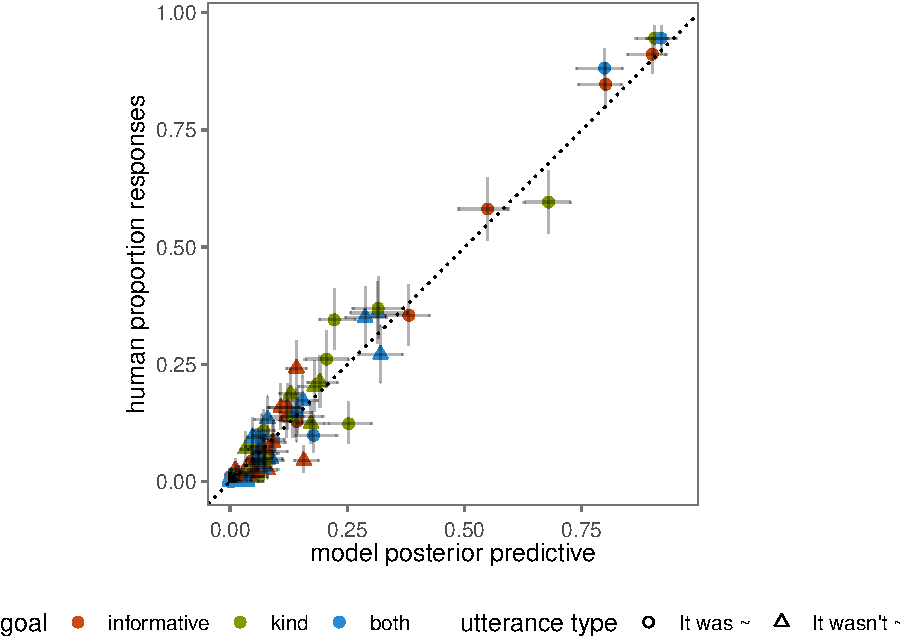
\includegraphics{polite_manuscript_files/figure-latex/variance-1.pdf}
\caption{\label{fig:variance}Full distribution of human responses vs.~model
predictions. Error bars represent 95\% confidence intervals for the data
(vertical) and 95\% highest density intervals for the model
(horizontal).}
\end{figure}

We hypothesized that speakers describing bad
states (e.g., Bob's performance deserved 0 hearts) while trying to be both
informative and kind would produce more indirect, negative utterances
(e.g., \enquote{It wasn't bad}).
% Such indirect speech acts serve to
% save the listener's face while also conveying a vague estimate of the
% true state.
This prediction was confirmed: a Bayesian mixed-effects
model predicting negation as a function of true state and goal yielded
an interaction such that a speaker with both goals to be informative and
kind produced more negation in worse states compared to a speaker with
only the goal to be informative (\emph{M} = -1.33, {[}-1.69, -0.98{]})
and goal to be kind (\emph{M} = -0.50, {[}-0.92, -0.07{]}).

Next, to connect the behavioral data to our model, we inferred the parameters of the RSA model (e.g., the speaker's utility weights in each goal condition; see Supplementary Materials) via a Bayesian data analysis \cite{lee2014}.
To approximate the semantics of the words as interpreted by the literal listener \(L_0\), we obtained literal meaning judgments from an independent group of participants (\emph{N}=51).
%Using an independent sample (\emph{N}=51), we measured judgments of how well different utterances apply to each of the levels on the heart scale (e.g., to what extent is \enquote{terrible} true of 2 out of 3 hearts?).
%These measurements were used to approximate the semantics of the words as interpreted by the literal listener \(L_0\).
Predictions from the full polite speaker model showed a very strong fit to participants' utterance choices (\(r^2\)(96) = 0.97; Figure \ref{fig:variance}).

We also compared the predictions of our model to its variants containing subsets of the three utilities in the full model. Both the variance explained and the marginal likelihood of the observed data were the highest for the full model (Table \ref{tab:comparisonTable}).
Only the full model captured the participants' preference for negation in the condition in which the speaker had both goals to be informative and kind about truly bad states, as hypothesized (Figure \ref{fig:comparison}). All three utilities -- informational, social, and presentational -- were required to fully explain participants' utterance choices.
The utility weights inferred for the full model (Table  \ref{tab:phi}) provide additional insight into how polite language use operates: our condition manipulation altered the balance between these weights, but all utilities played a role in all conditions.

% \emph{Being kind} requires equal weights on all three utilities, indicating that Gricean informativity needs to be part of language use even when it is explicitly not the goal.
% \emph{Being informative} pushes the weight on social utility close to zero, but the weight on \emph{appearing kind} stays high, indicating that speakers are expected to manage their own face even when they are not considering others'.
% \emph{Kind and informative} speakers emphasize honesty slightly more than kindness.
% In all cases, however, the presentational utilities have greatest weight, indicating perhaps that appearing honest and kind is more important than actually being so!

\begin{figure}
\centering
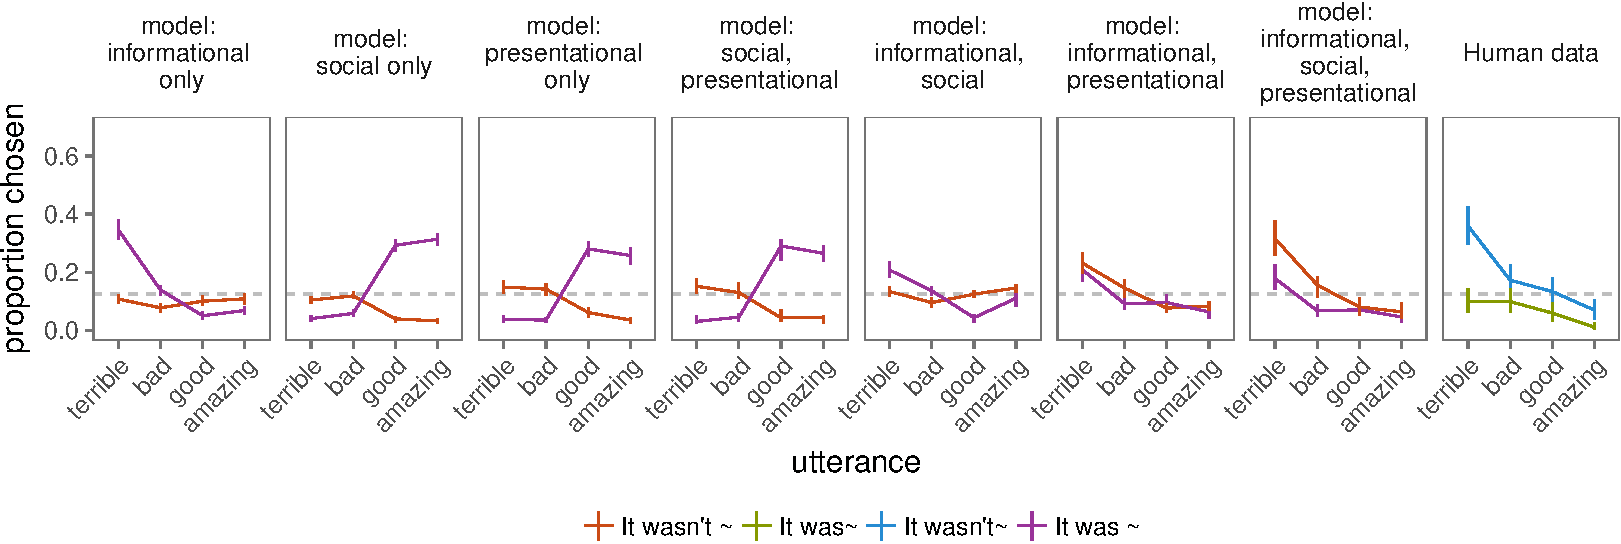
\includegraphics[width=\textwidth]{polite_manuscript_files/figure-latex/comparison-1.pdf}
\caption{\label{fig:comparison}Comparison of predictions for proportion of
utterances chosen by pragmatic speaker from possible model variants
(left) and human data (rightmost), given true state of 0 heart (on a scale
of 0 to 3) and speaker with both goals. Gray dotted line indicates
chance level at 12.5\%.}
\end{figure}

\begin{table}[tbp]
\begin{center}
\begin{threeparttable}
\caption{\label{tab:comparisonTable}Comparison of variance explained for each model variant and log Bayes Factors quantifying evidence in favor of the full model, in comparison to each of the alternatives.}
\begin{tabular}{lll}
\toprule
Model & \multicolumn{1}{c}{Variance
explained} & \multicolumn{1}{c}{log BF}\\
\midrule
model:
informational only & 0.83 & 274.89\\
model:
social only & 0.22 & 885.52\\
model:
presentational
only & 0.23 & 873.83\\
model:
social,
presentational & 0.23 & 864.00\\
model:
informational,
social & 0.92 & 25.06\\
model:
informational,
presentational & 0.96 & 11.14\\
model:
informational,
social,
presentational & 0.97 & 1.00\\
\bottomrule
\end{tabular}
\end{threeparttable}
\end{center}
\end{table}


%%%%%%%%%%%%%%%%%%
%%%%% Implications %%%%%%%
%%%%%%%%%%%%%%%%%%

% It is also possible, however, that culture affects the mapping between the world states and subjective values for the listener.
% Our formal modeling approach with systematic behavior measurements can help understand the vast range of politeness practices found across languages.
To precisely estimate choice behavior, our experiment abstracted away from
natural interactions in a number of ways. Real speakers have access to a potentially infinite range of utterances to manage the tradeoffs in our experiment (\enquote{It's hard to write a good poem}, \enquote{That
metaphor was so relatable!}). Under our framework, each utterance will have strengths and weaknesses relative to the speaker's goals. Computation in an unbounded model presents technical challenges \cite{goodman2016} (perhaps paralleling the difficulty human speakers feel in finding the right thing to say in a difficult situation).

%Our work extends previous models of language beyond standard informational utilities to address social and self-presentational concerns.
%Previous theories of language use have not explained how informational versus social concerns trade off to inform the speaker's utterance choices.

For a socially-conscious speaker, managing listeners' inferences is a fundamental task. Inspired by the theory of politeness as face management \cite{brown1987}, our model takes a step towards understanding it.
By considering utility-driven inferences in a social context \cite{baker2017rational, hamlin2013mentalistic},
our approach here could give insights into a wide range of social behaviors beyond speech. And by experimenting with different utility weights and value functions, our model could provide a framework for understanding systematic cross-cultural differences in what counts as polite.

Politeness is only one of the ways that language use deviates from pure information transfer. When we flirt, insult, boast, and empathize, we also balance being informative with goals to affect others' feelings and present particular views of ourselves. Our work shows how social and self-presentational motives can be integrated with other concerns more generally, opening up the possibility for a broader theory of social language. Further, a formal account of politeness moves us closer to courteous computation -- to computers that can communicate with tact.


%In sum, this work takes a concrete step toward quantitative models of the nuances of human speech.
% Your references go at the end of the main text, and before the
% figures.  For this document we've used BibTeX, the .bib file
% scibib.bib, and the .bst file Science.bst.  The package scicite.sty
% was included to format the reference numbers according to *Science*
% style.

%BibTeX users: After compilation, comment out the following two lines and paste in
% the generated .bbl file.

\bibliography{politeness}

\bibliographystyle{Science}





\section*{Acknowledgments}
All authors designed research and wrote the paper;
E.J.Y. and M.H.T. performed research and analyzed data.
Our model,
preregistration of hypotheses, procedure, data, and analyses are available at
\url{https://github.com/ejyoon/polite_speaker}.
The authors declare no conflict of interest.
This work was supported by NSERC PGS Doctoral scholarship
PGSD3-454094-2014 to EJY, NSF Graduate Research Fellowship DGE-114747 to
MHT, ONR grant N00014-13-1-0788 to NDG, and NSF grant BCS 1456077 to
MCF.

%Here you should list the contents of your Supplementary Materials -- below is an example.
%You should include a list of Supplementary figures, Tables, and any references that appear only in the SM.
%Note that the reference numbering continues from the main text to the SM.
% In the example below, Refs. 4-10 were cited only in the SM.
\newpage


%References \textit{(4-10)}


% For your review copy (i.e., the file you initially send in for
% evaluation), you can use the {figure} environment and the
% \includegraphics command to stream your figures into the text, placing
% all figures at the end.  For the final, revised manuscript for
% acceptance and production, however, PostScript or other graphics
% should not be streamed into your compliled file.  Instead, set
% captions as simple paragraphs (with a \noindent tag), setting them
% off from the rest of the text with a \clearpage as shown  below, and
% submit figures as separate files according to the Art Department's
% instructions.


%\clearpage
%
%\noindent {\bf Fig. 1.} Please do not use figure environments to set
%up your figures in the final (post-peer-review) draft, do not include graphics in your
%source code, and do not cite figures in the text using \LaTeX\
%\verb+\ref+ commands.  Instead, simply refer to the figure numbers in
%the text per {\it Science\/} style, and include the list of captions at
%the end of the document, coded as ordinary paragraphs as shown in the
%\texttt{scifile.tex} template file.  Your actual figure files should
%be submitted separately.

\end{document}
